\section{Architecture and Implementation}

\subsection{\texttt{SVDLinear} Layer Design}
Compressed projections are implemented via the custom \texttt{SVDLinear} class, which executes:
\[
y = (x V^\top) U^\top + \frac{\alpha}{r_{\text{lora}}} (x A_{\text{lora}}^\top) B_{\text{lora}}^\top + b
\]
By factoring $W$ into $U \in \mathbb{R}^{d_{\text{out}} \times r}$ and $V \in \mathbb{R}^{r \times d_{\text{in}}}$, intermediate tensor dimensions drop from $d_{\text{out}}$ to bottleneck rank $r$.

\begin{figure}[H]
\centering
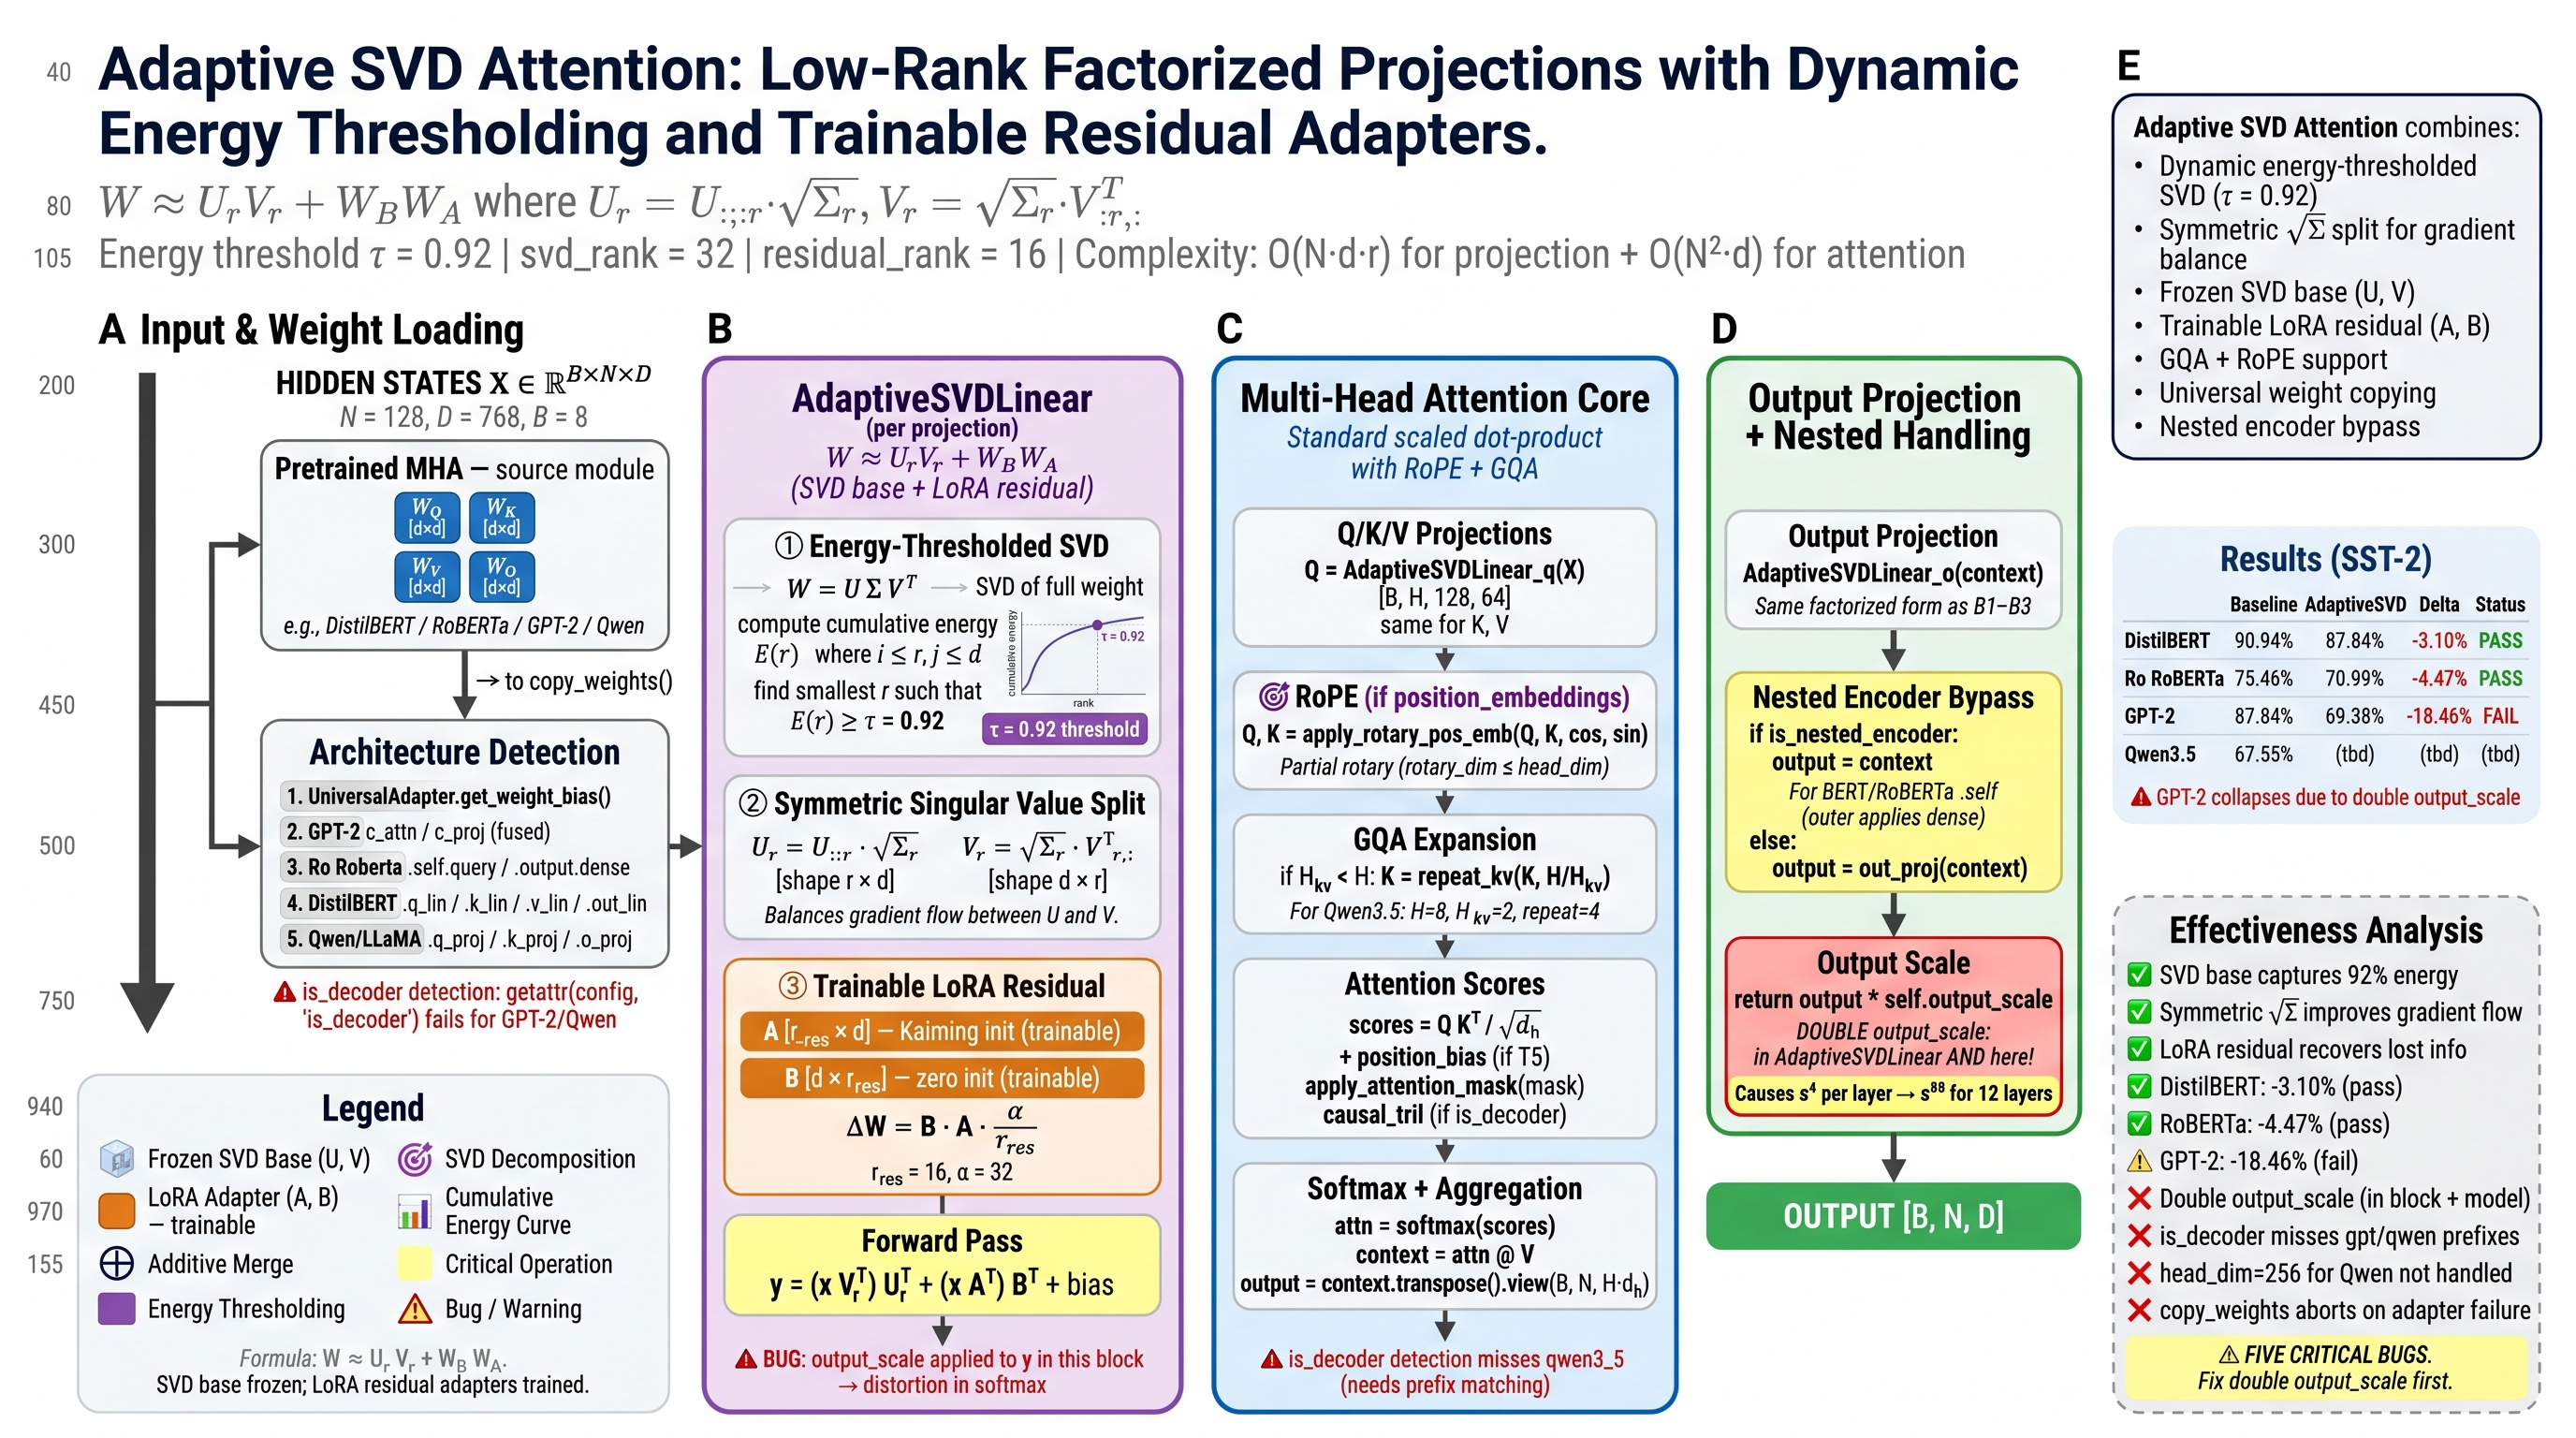
\includegraphics[width=0.85\linewidth]{figures/adaptivesvd.jpeg}
\caption{Factorized \texttt{SVDLinear} architecture replacing monolithic dense projections.}
\label{fig:arch_aa_svd}
\end{figure}
